\documentclass[tikz,border=0pt]{standalone}
\usepackage{amsmath}
\usetikzlibrary{arrows.meta,positioning,calc}

\begin{document}
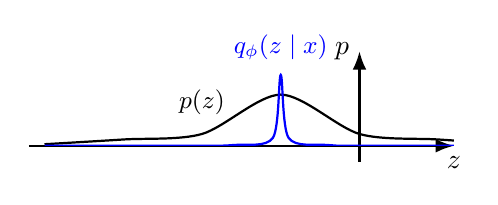
\begin{tikzpicture}[
    >=Latex,
    small/.style={font=\small},
]

% Left: AE latent (unconstrained, irregular)
% \begin{scope}[shift={(0,0)}]
%     \draw[->,thick] (-2.1,0) -- (2.2,0) node[below] {$z_1$};
%     \draw[->,thick] (0,-2.1) -- (0,2.2) node[left] {$z_2$};
%     \node[small] at (0,2.55) {AE latent (unregularized)};

%     % an irregular "cloud"
%     \fill[black!15] (-1.4,0.9) .. controls (-1.9,0.2) and (-1.3,-0.9) .. (-0.5,-1.1)
%                   .. controls (0.2,-1.3) and (1.4,-0.9) .. (1.6,-0.1)
%                   .. controls (1.9,0.8) and (1.0,1.6) .. (0.2,1.4)
%                   .. controls (-0.4,1.3) and (-0.9,1.4) .. (-1.4,0.9) -- cycle;
%     \draw[thick] (-1.4,0.9) .. controls (-1.9,0.2) and (-1.3,-0.9) .. (-0.5,-1.1)
%                   .. controls (0.2,-1.3) and (1.4,-0.9) .. (1.6,-0.1)
%                   .. controls (1.9,0.8) and (1.0,1.6) .. (0.2,1.4)
%                   .. controls (-0.4,1.3) and (-0.9,1.4) .. (-1.4,0.9) -- cycle;

%     \node[small, align=center] at (0,-2.65)
%     {$z$ distribution is unknown\\hard to sample reliably};
% \end{scope}

% Right: VAE latent (regularized to N(0,I))
% \begin{scope}[shift={(6.6,0)}]
%     \draw[->,thick] (-2.1,0) -- (2.2,0) node[below] {$z_1$};
%     \draw[->,thick] (0,-2.1) -- (0,2.2) node[left] {$z_2$};
%     \node[small] at (0,2.55) {VAE latent (KL-regularized)};

%     % Gaussian-ish density rings
%     \foreach \r/\a in {0.4/25,0.8/18,1.2/12,1.6/7,2.0/3}{
%         \draw[black!\a, thick] (0,0) circle (\r);
%     }
%     \fill[black!25] (0,0) circle (0.12);
%     \node[small, align=center] at (0,-2.65)
%     {$q_\phi(z\mid x)$ pushed toward\\$p(z)=\mathcal N(0,I)$};
% \end{scope}

% Bottom: narrow posterior intuition
\begin{scope}%[shift={(3.3,-6.0)}]
    % axes
    \draw[->,thick] (-4.2,0) -- (1.2,0) node[below] {$z$};
    \draw[->,thick] (0,-0.2) -- (0,1.2) node[left] {$p$};
\clip (-4.2,0) rectangle (1.2,1.5);
    % wide prior
    \draw[thick] plot[smooth] coordinates {(-4,0.02) (-3,0.08) (-2,0.15) (-1,0.65) (0,0.15) (1,0.08) (2,0.02) (3,0.01) (4,0.005)};
    \node[small] at (-2,0.55) {$p(z)$};

    % narrow posterior around some mean
    \draw[thick,blue] plot[smooth] coordinates {(-4,0.0) (-2.2,0.0) (-1.6,0.01) (-1.1,0.1) (-1.0,0.9) (-0.9,0.1) (-0.4,0.01) (0.2,0.0) (4,0.0)};
    \node[small,blue] at (-1,1.25) {$q_\phi(z\mid x)$};
\end{scope}

\end{tikzpicture}
\end{document}


